\documentclass{article}


\usepackage{arxiv}

\usepackage[utf8]{inputenc} % allow utf-8 input
\usepackage[T1]{fontenc}    % use 8-bit T1 fonts
\usepackage{hyperref}       % hyperlinks
\usepackage{url}            % simple URL typesetting
\usepackage{booktabs}       % professional-quality tables
\usepackage{amsfonts}       % blackboard math symbols
\usepackage{nicefrac}       % compact symbols for 1/2, etc.
\usepackage{microtype}      % microtypography
\usepackage{lipsum}
\usepackage{graphicx}

\title{CouncilFS: An Incentivized, Resilient File Distribution System}


\author{
  Gabrielle Beck \\
  Department of Computer Science\\
  Johns Hopkins University \\
 Baltimore, MD \\
  \texttt{becgabri@jhu.edu} \\
  %% examples of more authors
   \And
 Tushar Jois \\
  Department of Computer Science\\
  Johns Hopkins University\\
  Baltimore, MD \\
  \texttt{jois@cs.jhu.edu} \\
  %% \AND
  %% Coauthor \\
  %% Affiliation \\
  %% Address \\
  %% \texttt{email} \\
  %% \And
  %% Coauthor \\
  %% Affiliation \\
  %% Address \\
  %% \texttt{email} \\
  %% \And
  %% Coauthor \\
  %% Affiliation \\
  %% Address \\
  %% \texttt{email} \\
}

\begin{document}
\maketitle

\begin{abstract}
  We present \textsc{CouncilFS},
\end{abstract}


% keywords can be removed
%\keywords{First keyword \and Second keyword \and More}


\section{Introduction}

The main purpose of this work is to try and solve the inherent wastefulness in
popular cryptocurrencies by proposing a proof of work that can be used to
perform a useful function, in this case, storing files for those who are willing
to pay for such storage. Other blockchain researchers before us have also
identified this as a problematic issue and have tried to rectify it through
creating alternatives to Bitcoin’s hash-based puzzle. These solutions include
schemes that do not rely on ludicrous amounts of computation such as Proofs of
Stake (where who gets to mine is based off of players that have more stock in
the current network) and Proofs of Space (where there is a lot of computation
done up front for initialization of a new miner, but the actual mining itself is
cheap). However, schemes that do not rely on heavy computation tend to suffer
from ``nothing at stake'' problems because there is no incentive for miners to
work on just the longest chain when it is so inexpensive to try and extend other
forks.

Therefore, the other alternative to these style of proofs are proofs of
work that serve some utilitarian function (i.e. distributed file storage).
Proofs of Retrievability (PoRs) have been proposed as alternatives to a hash
based proof of work by authors such as the creators of Permacoin, however, there
scheme has some limitations in that they assume that the file has to be publicly
available and that it can be handed out to new miners by a trusted dealer. This
limits its usefulness. Because they focus on storing a large publicly known
file, they also do not acknowledge any potential that this scheme brings for
loose censorship resistance. By distributing the trusted dealer among more
mutually distrusting parties, we can accommodate the storage of encrypted files
and provide a myriad of parties that a client can access should any few be
blocked or taken down. Overall, we believe our scheme leverages economic
incentives and blockchain technologies to create a currency that can more or
less be used to drive distributed storage in a way that penalizes those that
attempt to cheat clients out of money without of their files and allows for
discrete sharing of potentially covert information.

\paragraph{Contributions.} We present \textsc{CouncilFS}, a file distribution
system with censorship-resistant properties. These properties are incentivized
with a blockchain-based system that provides payment for distribution services
rendered. Our contributions are the following:
\begin{itemize}
\item A new file distribution system that uses a two-level node hierarchy to
  bootstrap trust and a blockchain to provide incentives.
\item A protocol that combines proofs-of-retrieveability, with the
  notion of payment channels to provide incentivized 
\item The implementation the proofs-of-retrieveability, client, and alderman
  code of \textsc{CouncilFS} in the Go programming language.
\end{itemize}

\section{Related Work}
\subsection{Alternative Proofs of Work}
Our work exists at the cross-section of many different active fields of research. Before this paper, there have been many proposals for Proof-of-Work schemes that serve some useful function or purpose like PrimeCoin. In a previous paper, there has also been a proposal to utilize a POR as a proof of work for the purpose of storing archival information that would be known by all miners so that validation of the files could be assured $\mathcal{D}$. The authors also assume that this file would not be updated and introduce a new stateful signature scheme that should be relatively efficient while also ensuring that a miner cannot "outsource" their computation. This differs from our scheme as we allow for the existence of other files carried by clients that are given directly to trusted nodes, called \emph{Alderman}, and are not verifiable by every single node on the network.\\

Other alternative proofs of work that are similar to PORs include Proofs of Space, Proofs of Data Possession and Proofs of Erasure. Proofs of Space, for example, guarantee that a miner is holding some space it could be doing computation open and then answer challenges to ensure this is in fact the case. The way this scheme is commonly implemented is to use a form of pebbling and pebble the spaces and prove something about the graph to a verifier. One popular Proof of Space is spacemint which is unique in that it implements two different blockchains and utilizes a punishment mechanism to disincentivize miners from deviating from the protocol in ways that are unlikely to happen if Proof of Work algorithms (for example, nothing at stake problems and block/challenge grinding). In our future work, we propose a similar kind of punishment mechanism. However, we use this tool to demote misbehaving \emph{Alderman} and to provide recompense for grief-stricken clients. We do not propose two different blockchains/ledgers for history either.

\subsection{Censorship Resistant File Storage}
There has also been work done previously in the creation of file storage resistant to the takedown of particular governments and agencies. Publius, for example, was proposed as a method of resistance in which n servers host the encrypted content but in order to get the key a client must obtain k-out-of-n secret shares that are also controlled by these servers. While there is plausible deniability on the part of the servers, as they are hosting encrypted material, there is no mechanism or recompense in place for servers electing to delete their shares and no way to communicate this information to all of the other servers readily on the network. What this paper attempts to do is fundamentally different as we not only want to provide a mechanism by which servers can help dissidents/clients but we want to provide them an incentive to do so as well. Namely, in the form of currency. 

\section{Construction}

\subsection{Overview}

There are three types of nodes in our network: \emph{members}, \emph{aldermen},
and \emph{clients}. Members form the backbone of the network; they are the nodes
that primarily interface with the blockchain. They verify transactions between
users of the underlying currency of \textsc{CouncilFS}. Aldermen are members of the
network who have been elected to take on more responsbility in the network.
Their primary responsibility is to maintain instances of the files that clients
upload. Clients pay for this privlege, and engage in a protocol to ensure that
the alderman remains honest. Aldermen who are not honest are demoted back to the
member pool. This general outline of our construction is discussed in more
detail in the subsections below.

\subsection{Members}

At the core of the \textsc{CouncilFS} network are members. The underlying token
of \textsc{CouncilFS}, known as a \emph{shire}, is exchanged between users as
transactions. Members organize user transactions into blocks, verify
correctness, and perform a proof-of-work computation. The computation performed
is then compared to a difficulty value by all other nodes, and if it is less
than this value, the rest of the network accepts a member's block. This process,
known as Nakamoto Consensus, is analgous to the process performed by miners in
Bitcoin \cite{btc}.

\subsubsection{Proofs-of-Retrievability}

Unlike Bitcoin miners, however, \textsc{CouncilFS} members perform a
proof-of-retrieveability (PoR), in which a prover proves that they are able to
retrieve a file on demand, without transmitting the entire file to a the
verifier. This PoR is performed by every member on a common dataset
$\mathcal{D}$; because this dataset is common, each other member in the network
acts a verifier. The PoR is computationally intensive, and is still
fundamentally a proof-of-work scheme; it acts as a replacement for the SHA-256
hash function used in Bitcoin and related cryptocurrencies.

Our instantiation of PoR is similar to the one used in Permacoin \cite{perma},
in that it acts as a positive use of computational resources. There are some key
differences, however. In \textsc{CouncilFS}, the aldermen replace the dealer as
the arbiter of the common dataset. The aldermen decide which members get which
slices of $\mathcal{D}$, rather than having a trusted setup phase. Additionally,
because the aldermen handle $\mathcal{D}$, it can be updated continuously. Both
of these points are discussed further later in the paper.

\begin{figure}[t]
  \centering
  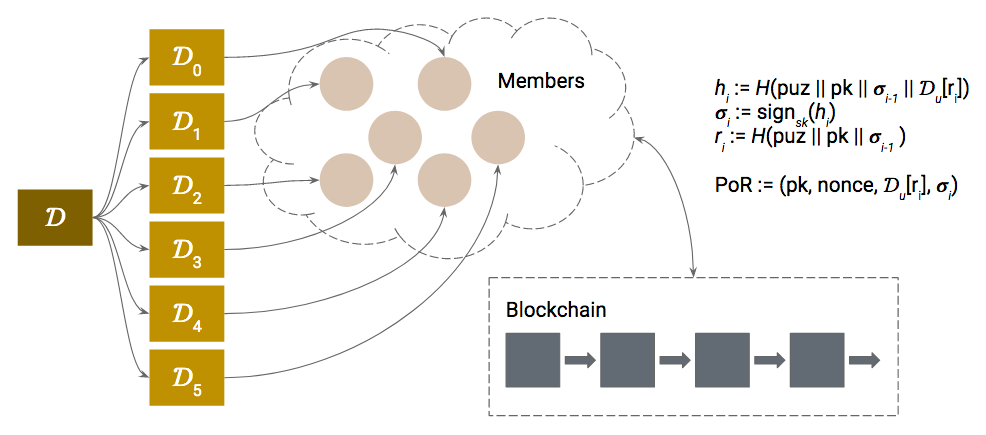
\includegraphics[width=\linewidth]{figures/por_member.png}
  \caption{Structure of the PoR employed by a member.}
  \label{fig:por-member}
\end{figure}

\subsection{Aldermen}

Aldermen constitute the second tier of nodes in \textsc{CouncilFS}. These nodes
are trusted by the others in the network to provide file distribution and
logistics services for all of \textsc{CouncilFS}. File storage capabilities are
provided to \emph{clients}, who pay the aldermen for this distribution service.
Other nodes in the network can download files from the aldermen as long as this
payment is made. For the members, the provide the common data store used in the
PoR. This extra responsibility requires trust, which is bootstrapped by the
escrow of shire tokens and by a selection process. In addition to the shire
clients pay to store files, aldermen (as a pool) earn 15\% of the block reward
from a newly-mined block for the additional responsibility they take on from the
network. This two-level system is similar to the concept of ``masternodes'' in
cryptocurrencies such as Dash \cite{dash-coin}, but aldermen in
\textsc{CouncilFS} have different responsibilities and additional sources of
income other than a part of the block reward.

\subsubsection{Selection}

The selection process defines how an member becomes an alderman. A member
becomes an alderman after posting a \emph{selection transaction} to the
blockchain. Such a transaction validates that the member has met the
prerequisites for becoming an aldermen. After this transaction is confirmed in
the blockchain (\emph{i.e.}, deep in the longest chain), then the other aldermen
consider the member an alderman.

The biggest prerequisite for joining the network is the accumulation of 100,000
shire. This significant investment ensures that the alderman participates in the
network correctly, as the value of their investment fluctuates with the success
of the network. It also restricts the possibility of a Sybil attack to
compromise the alderman network. Because of the fixed growth rate of shire (in a
typical implementation), there will be a limit on the total number of

There are also practical requirements for the aldermen to satisfy. One of them
is to maintain strong bandwidth and a static IP address. This allows for members
to download the common data store for PoRs and for clients to upload and
download files, as described below. They also must respond to pings on their IP
address to demonstrate liveness. The alderman should also have sufficient disk
space to store files; the aldermen must store the entire common data store and
(potentially) the files that clients wish to upload.

\subsubsection{Common Data Store $\mathcal{D}$}

Aldermen are responsible for handling and dividing up the common data store
$\mathcal{D}$. This dataset is something with high public value, such as data
from the Internet Archive or from Wikipedia. Each alderman holds a full copy of
this dataset, split into shards. When a member wishes to join
\textsc{CouncilFS}, the alderman gives specific shards to the new member based
on the current state of the network. Aldermen attempt to distribute the file
randomly, such that all shards of $\mathcal{D}$ are equally distributed.

The dataset cannot be updated in place. This is because changes to the dataset
may break the validity of PoRs already on the blockchain. However, the dataset
can be appended to, as members are only given shards of the full dataset to
store. When the members wish to operate on the new segments that were appended
to $\mathcal{D}$, they simply download them from the aldermen.

\subsubsection{Client File Channels}

\begin{figure}[t]
  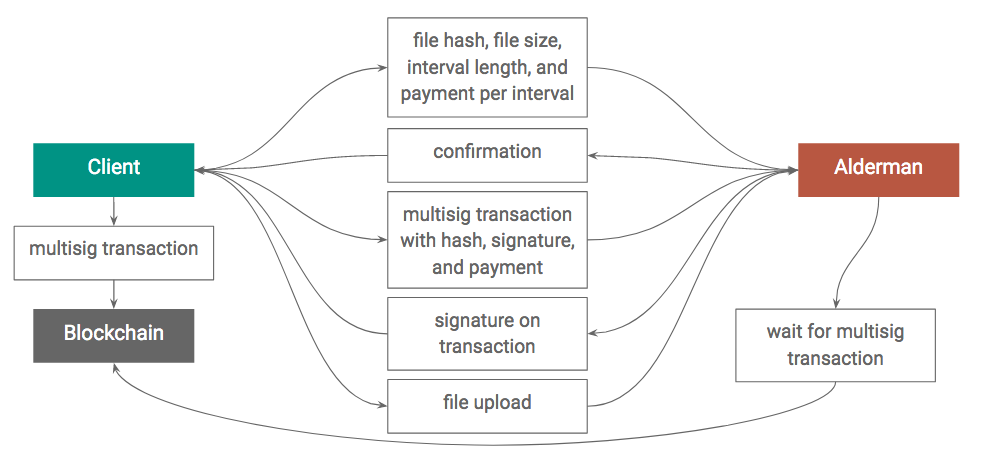
\includegraphics[width=\linewidth]{figures/init_channel.png}
  \caption{Initializing a file channel between a client and an alderman.}
  \label{fig:channel}
\end{figure}

The primary service aldermen provide is a file distribution network for hire.
Clients engage in a protocol in order to upload a file and provide a constant
flow of payment to an alderman This
protocol, known as a \emph{file channel}, is similar to the off-chain
transactions developed in previous work such as the payment channels in the
Lightning Network \cite{lightning}. However, in addition to the payment being
sent across the channel, the client verifies that the alderman is holding the
file by performing a PoR for it across the same channel. We use ECDSA in order
to cryptographically verify the communication between a client and an alderman.
The initialization part of the protocol is shown in Figure \ref{fig:channel}.

\paragraph{Initialization.} When a client wishes to upload a file to an
alderman, they broadcast the file hash, file size, interval length, and payment
per interval. The interval is defined in nanoseconds, and refers to the amount
of clock time that passes before the next payment from the client. The client
can optionally send the number of intervals that the file should be held
(\emph{i.e.}, the total amount of time spent with the file). These parameters
allow an alderman to decide if it is worth their time to store the file the
client offers to publish. Aldermen that wish to accept the offer send replies to
the client that state their intent to serve the file. If they wish to counter
the offer, they can send a response with potential changes to the payment.

After this negotiation between a client and an alderman, the two parties proceed
to the funding phase. The client creates a 2-of-2 multisig transaction, in which
both the client and the alderman need to sign the transaction before it is
accepted as valid. This transaction contains the hash of the file being
uploaded, the signature on the hash, and the payment parameters of the channel.
It also defines how much of the client's shire will be held in escrow during the
channel. If the ``file'' being uploaded is actually the sharded form of a full
file, this transaction may optionally include the transaction locations of the
other shards that compose this file. The client then sends this transaction to
the alderman directly (without broadcasting it) who signs the transaction if the
client set the parameters properly.

The client broadcasts the transaction to the members. Once the transaction is
sufficiently deep in the blockchain, the protocol moves into the upload phase.
The client sends the file to alderman, who stores it on disk after verifying
the signature on the file. If this signature verification fails or if the file
is not uploaded in time, the alderman forgets the channel. Else, the alderman
notifies the client of a successful upload and the channel enters normal operation.

\paragraph{Operation.} During normal operation, before the current interval has
expired, the client requests a PoR for the file from the alderman in the open
channel. The alderman sends a PoR for the file back to the client, and the
client verifies it. If the verification succeeds, the client sends a new 2-of-2
multisig transaction that updates the payment to use the escrow funds to pay the
alderman. The alderman, on receipt of the transaction, resets the interval count
and holds the uploaded file on disk.

\paragraph{Closure.} If the client sends a closure request, the alderman decides
that it cannot hold the file anymore, or if the timeout for payment expires, the
channel moves to a closed state. Either party can initiate the closure by
posting the latest multisig transaction from the channel to the blockchain. When
this occurs, the client will cease sending payments to the alderman, and the
alderman will delete the file from disk. Ordinarily, the closing party will
notify their counterparty in order to have a clean finish to the channel.
However, if they do not do this, the counterparty can still know the channel is
closed, as they can check the blockchain for one of the transactions sent as
payment in the channel.

\subsubsection{File Retrieval}

Allowing other users of \textsc{CouncilFS} to download files is one of the
responsibilities of aldermen. The transaction ID of the funding transaction is
the only information necessary to find a file, since a user can read off the
authentication information (such as signature and uploader public key) along
with location in the alderman network (alderman public key) directly off the
blockchain. In practice, the client can post the absolute location of the
funding transaction so other users do not have to iterate through the whole
blockchain to find file information.

Based on the selection criteria denoted above, every alderman must have a static
IP address that is recorded on chain. So, once the user finds the location of
the file, they can resolve the IP address associated with that public key by
looking on the blockchain. They then use that IP address to make a request to
the alderman for a file pointed to by a particular transaction ID. The alderman,
using its mapping of transaction IDs to channels, finds the file to which the ID
refers and retrieves it for the user.

The user can assume that the file referenced by a funding transaction is
available at the alderman until a payment transaction is posted to the
blockchain. This parallels the state of the file channel between a client and an
alderman: it opens when the funding transaction is posted, and closed when a
payment transaction is posted. If the alderman is in the middle of receiving or
deleting a file, it can return such a status to the user, even if the
transaction that supports this claim has not been posted to the chain. 

Note that this structure means that client does not need to strictly have the
file on disk in order to validate the file during normal channel operation
(above). They can request the file from the alderman as a normal user and verify
it against both the signature stored on the blockchain and the PoR sent over by
the alderman. This alternative method, although more bandwidth-intensive, is
useful as a tool against censorship; a client can send a restricted document to
an alderman and retrieve it when it is safe to do so.


\subsubsection{Punishing Misbehavior}

An alderman is expected to behave according to the norms of the protocol. When
an alderman starts misbehaving, it is in the best interest of the rest of the
alderman if they catch the misbehavior (assuming the majority of aldermen are
honest). A deeper analysis of the incentives surrounding alderman behavior is in
the Discussion section below.

\paragraph{Client-side.} A client can detect alderman misbehavior easily. There
are two ways alderman can misbehave: not storing the file provided by the client,
and not allowing user downloads of the file. Clients can issue challenges to
isolate misbehavior. Implicit to this challenge process is the determination of
liveness, as a dead alderman will not respond to a challenge fast enough.

In the first misbehavior case, the alderman does not hold the uploaded file.
This however, is easily detectable: if the PoR sent across the channel during a
payment interval does not validate, the client can simply close the channel.
Thus, the alderman no longer gets paid, as it did not perform the service as
negotiated. In the second case, users cannot download the file as held by the
alderman. In order to detect this, other users should notify the client
out-of-band that this is occurring, or the client can verify for themselves by
attempting to download the full file from the alderman during a payment
interval. Once again, if the alderman fails this challenge, the client can
simply close the channel.

Blacklisting is a powerful tool that clients have to punish chronic misbehavior.
If an alderman continues to cheat clients, clients can stop responding to their
offers, and add them to a blacklist. As more and more clients add said alderman
to their blacklists, the alderman is effectively shunned from the network due to
their behavior. This means the significant resources the alderman devoted to
selection goes to waste as a result of this punishment.

\paragraph{Alderman-side.} Aldermen determine misbehavior by challenging each
other on the operations of the network. If an alderman can prove to a challenger
that it is meeting the requirements of the protocol, it can remain in the
network; otherwise, it is punished by being sent back to the member pool. This
type of punishment is even more severe, as it is enforced by the protocol
itself.

To detect misbehavior, aldermen challenge each other on the files they store. To
achieve the property of resiliency, clients will replicate their file across
several aldermen. Other aldermen can detect this by reading the file information
off the blockchain, by looking at the funding transaction for a file channel.
Additionally, aldermen challenge each other on the common dataset $\mathcal{D}$
that they distribute to the members of the protocol.

Every block, two \emph{boards} of aldermen are selected. The first board, Board
A, checks every node on in the second board, Board B. The first check they
perform is a ping check to verify the alderman is up and responsive. The next
check is to retrieve a client's file from the alderman. The final check is a
PoR on $\mathcal {D}$, which Board A should already have a copy. Every passed
check gives an alderman \emph{merits}, while failed ones take merits away. At a
certain threshold of merits, the alderman is kicked back to the general member
pool.

The random selection of the boards ensures that the attacker must be selected
every time in order to continuously trick the system. As such, this probabilistic
nature makes attacks against the alderman pool very unlikely. More checks can be
added as the network evolves. This structure is inspired by proofs-of-service
\cite{proof-of-service} found in other cryptocurrencies. \textsc{CouncilFS} goes
beyond this by requiring nodes to not only be online, but actively participating
in the greater functionality of the network.

\section{Evaluation}

\subsection{Implementation}

We chose to implement the proof-of-retrieveability, client code and alderman
code of \textsc{CouncilFS}. These three aspects form the bulk of the novel ideas
of our construction. We did not implement a full blockchain, as our design is
agnostic to the underlying implementation of the transaction ledger. Our
requirements on the blockchain are that (1) it supports the types of
transactions outlined in our construction above, and (2) is structured to allow
PoRs are the source of the proof-of-work. An implementor would only have to fill
the necessary function stubs in our code in order to connect the blockchain
implementation to the rest of \textsc{CouncilFS}.

In the implementation, we employ a Reed-Solomon coding \cite{reed} in order to
encode data into shards. We choose this as it is a efficient distance-separable
code that allows up to have redundancy, which is especially important for
splitting $\mathcal{D}$ for distribution among the members. The encoding
functionality is also available to clients, so they can redundantly split the
file they wish to upload across several aldermen seamlessly. 

The source code for \textsc{CouncilFS} is written in the Go programming
language \cite{golang}. The memory and type safety as well as the speed of Go make it a good
fit for the implementation. The code has been released under the MIT license,
and is available at the GitHub repository found at:
\begin{center}
  \url{https://github.com/tusharjois/councilfs}
\end{center}


\subsection{Microbenchmarks}

\section{Discussion}

\paragraph{Incentive Structure.} Significant investment, so play by the rules

\paragraph{Replication and Censorship Resistance.} Delegation?

\paragraph{Trusting Aldermen.} Privacy concerns -- encryption

\paragraph{Updating $\mathcal{D}$.}

\paragraph{Future Work.}

\section{Conclusion}

\section{Examples of citations, figures, tables, references}
\label{sec:others}
 \cite{permacoin-repurposing-bitcoin-work-for-data-preservation}

Of note is the command \verb+\citet+, which produces citations
appropriate for use in inline text.  For example,
\begin{verbatim}
   \citet{hasselmo} investigated\dots
\end{verbatim}
produces
\begin{quote}
  Hasselmo, et al.\ (1995) investigated\dots
\end{quote}

\begin{center}
  \url{https://www.ctan.org/pkg/booktabs}
\end{center}


\subsection{Figures}
\lipsum[10] 
See Figure \ref{fig:fig1}. Here is how you add footnotes. \footnote{Sample of the first footnote.}
\lipsum[11] 


\subsection{Tables}
\lipsum[12]
See awesome Table~\ref{tab:table}.

\begin{table}
 \caption{Sample table title}
  \centering
  \begin{tabular}{lll}
    \toprule
    \multicolumn{2}{c}{Part}                   \\
    \cmidrule(r){1-2}
    Name     & Description     & Size ($\mu$m) \\
    \midrule
    Dendrite & Input terminal  & $\sim$100     \\
    Axon     & Output terminal & $\sim$10      \\
    Soma     & Cell body       & up to $10^6$  \\
    \bottomrule
  \end{tabular}
  \label{tab:table}
\end{table}

\subsection{Lists}
\begin{itemize}
\item Lorem ipsum dolor sit amet
\item consectetur adipiscing elit. 
\item Aliquam dignissim blandit est, in dictum tortor gravida eget. In ac rutrum magna.
\end{itemize}


\bibliographystyle{unsrt}  
\bibliography{references}  %%% Remove comment to use the external .bib file (using bibtex).
%%% and comment out the ``thebibliography'' section.


%%% Comment out this section when you \bibliography{references} is enabled.
%\begin{thebibliography}{1}

%\bibitem{kour2014real}
%George Kour and Raid Saabne.
%\newblock Real-time segmentation of on-line handwritten arabic script.
%\newblock In {\em Frontiers in Handwriting Recognition (ICFHR), 2014 14th
%  International Conference on}, pages 417--422. IEEE, 2014.

%\bibitem{kour2014fast}
%George Kour and Raid Saabne.
%\newblock Fast classification of handwritten on-line arabic characters.
%\newblock In {\em Soft Computing and Pattern Recognition (SoCPaR), 2014 6th
%  International Conference of}, pages 312--318. IEEE, 2014.

%\bibitem{hadash2018estimate}
%Guy Hadash, Einat Kermany, Boaz Carmeli, Ofer Lavi, George Kour, and Alon
%  Jacovi.
%\newblock Estimate and replace: A novel approach to integrating deep neural
% networks with existing applications.
%\newblock {\em arXiv preprint arXiv:1804.09028}, 2018.

%\end{thebibliography}


\end{document}
